\documentclass{article}
\usepackage[utf8]{inputenc}
\usepackage{amsmath}
\usepackage{graphics}

\title{Hello latex!}
\author{Marajul haque}
\date{jan 2025}

\begin{document}
	
	\maketitle
	
	\section*{introduction}
	
	Let's begin with a formula $e^{i\pi}+1=0$. 
	
	
	\begin{enumerate}
		
		\item As a \textbf{limit}
	
		
		$$ e=\lim_{n\to\infty}  \left(1+\frac{1}{n}\right)^n = \lim_{n\to\infty}\frac{n}{\sqrt{n!}}  $$
			
	
		
		\item We can do \underline {another}:
		
		$$ e=\sum_{n=0}^{\infty} \frac{1}{n!} $$
		
		
		\item As a  \textit{continued} fractions
		
		$$ e=2+\frac{1}{1+\frac{1}{\frac{1}{2+\frac{2}{3+\frac{3}{4+\frac{4}{5+\ddots}}}}}}$$
		
	\end{enumerate}
	
	\section{More formulas}
	
	
	$$\int_a^bf(x)dx$$
	
	\[\iiiint f(x,y,z)dxdydz\]
	
	$$ \iint f(x)dxdy$$
	$$\vec{v}=<v_1, v_2, v_3>  $$
	
	$$\vec{v}=\vec{v_1}+\vec{v_2}+\vec{v_3}$$
	
	$$\vec{v}\cdot\vec{w}$$
	$$ \vec{a}\times \vec{b}$$
	
	$$\begin{bmatrix} 
		
		1&2&3\\
		4&5&6\\ 
		7&8&9
		
	\end{bmatrix}
	$$	
	
	%\begin{center}
	
	%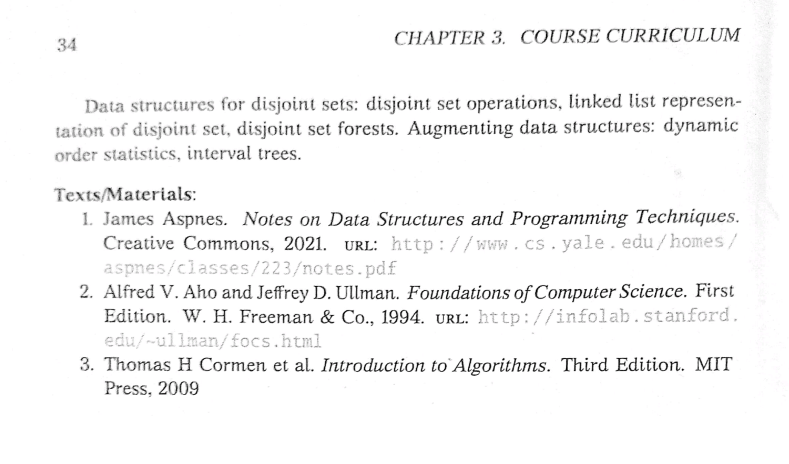
\includegraphics[width=0.5\textwidth]{gpt}
	%\end{center}
	
	
\end{document}
